%!TEX program = xelatex
\documentclass{ctexart}

\usepackage{style}

\title{龙卷风风场中输电塔结构的单向流固耦合分析}
\author{王勇}
\date{}

\begin{document}

\graphicspath{{figures/}}

\maketitle

\section{单向流固耦合分析基本框架}
单向流固耦合分析以解耦的方式进行\cite{benra2011comparison,qian2008fsi}:
首先,将结构表面视为刚性的流场壁计算流场的分布;
然后将流场计算得到的刚性壁压力施加到结构上以计算其响应。
单向流固耦合方法适用于结构在流场作用下变形较小(相比于流场的计算区域),
即流场的边界改变较小,几乎不影响流场的分布情况。

本文基于ANSYS Workbench平台进行输电塔底部二层结构在龙卷风风场中的单向流固耦合分析\cite{cornell2016fsi1, cornell2016fsi2},
基本流程见图\ref{fig:fsi-chart}所示。

\begin{figure}[!htpb]\label{fig:fsi-chart}
  \centering
  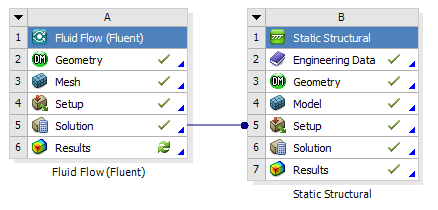
\includegraphics[width=0.6\textwidth]{fsi-chart.png}
  \caption{单向流固耦合分析流程图}
\end{figure}

\section{二层框架在龙卷风风场中单向流固耦合分析算例}

\subsection{建立结构实体模型}
流固耦合分析需要建立结构的实体模型才能实现流场计算结果向有限元网格的映射,
考虑到背景工程为钢管塔,
利用SolidWorks三维建模软件以面实体建立输电塔主要迎风构件(截面尺寸较大)、以线实体建立支撑等构件(截面尺寸较小,可忽略其迎风效应),如图\ref{fig:tower}所示。

\begin{figure}[!htpb]
  \centering
  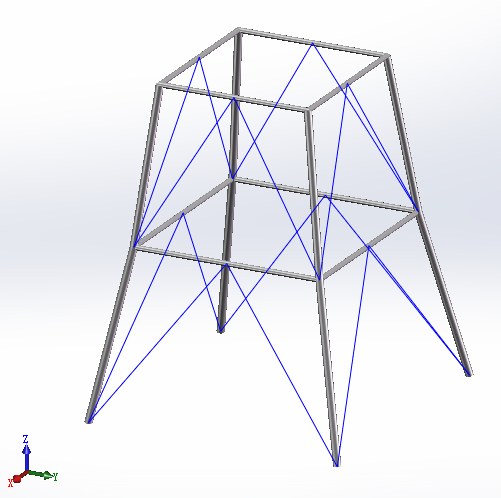
\includegraphics[width=0.6\textwidth]{tower.png}
  \caption{二层带支撑框架实体模型}
  \label{fig:tower}
\end{figure}


\subsection{龙卷风数值风洞}
在ANSYS Workbench中DesignModeler中建立考虑流固耦合的龙卷风数值风洞计算域。
基本流程为:导入结构面实体模型;由面实体生成其包围的实体;利用布尔运算从圆柱体减去该实体生成数值风洞计算域,如图\ref{fig:domain}所示。

\begin{figure}[!htpb]
  \centering
  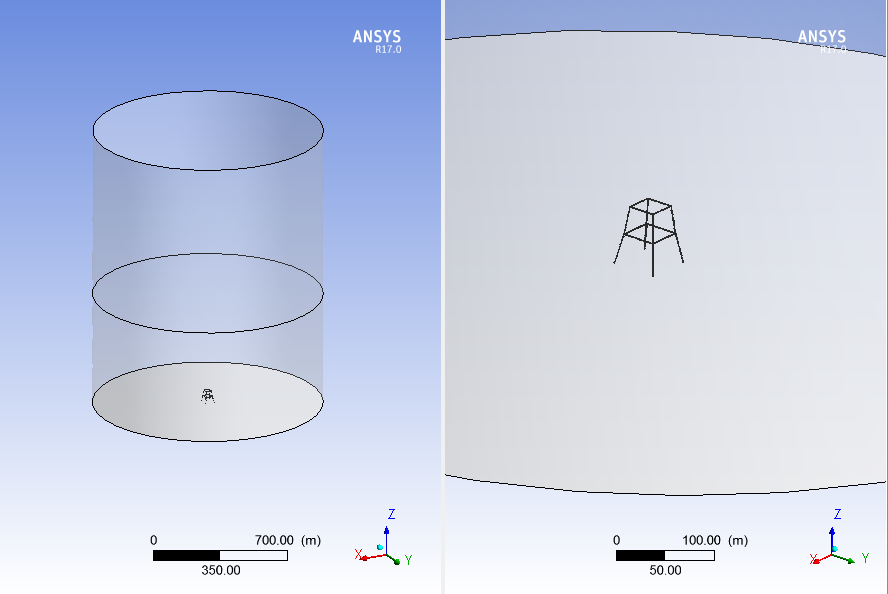
\includegraphics[width=0.6\textwidth]{domain.png}
  \caption{考虑流固耦合效应的龙卷风数值风洞计算域}
  \label{fig:domain}
\end{figure}

风洞计算域的基本尺寸为:
圆柱底面半径为\SI{600}{m},速度入口高度为\SI{600}{m},侧壁高度为\SI{900}{m}。
速度入口径向速度为\SI{14}{m/s},切向速度为\SI{8}{m/s}。

采用适应性较好的四面体进行网格划分,相应于结构表面的计算域边界面进行网格加密,并设置过渡层(inflation layer)。
计算流域网格在一层柱所在高度处的切面见图\ref{fig:fluid-mesh}(黑色部分为相应于结构柱的空洞)。

\begin{figure}[!htpb]
  \centering
  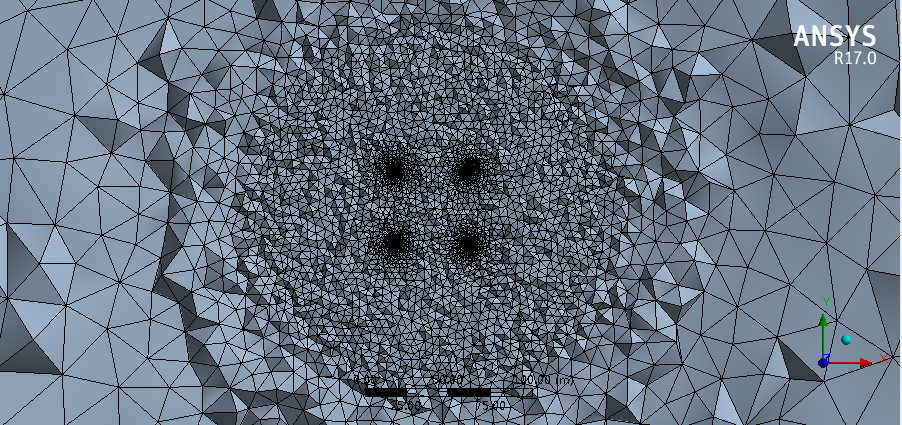
\includegraphics[width=0.6\textwidth]{fluid_mesh.png}
  \caption{计算流域网格切面图}
  \label{fig:fluid-mesh}
\end{figure}

\subsection{结构多尺度有限元模型}
在ANSYS Workben DesignModeler模块中为结构线实体赋予截面属性、在Mechanical模块中为面实体赋予厚度属性。
面实体以壳单元、线实体以梁单元进行有限元网格划分。
线实体端点(支撑的端点)与面实体端线(梁面或柱面的端线)的连接以多点约束单元MPC进行模拟\cite{wang2013tower},如图\ref{fig:mpc}所示。

\begin{figure}[!htpb]
  \centering
  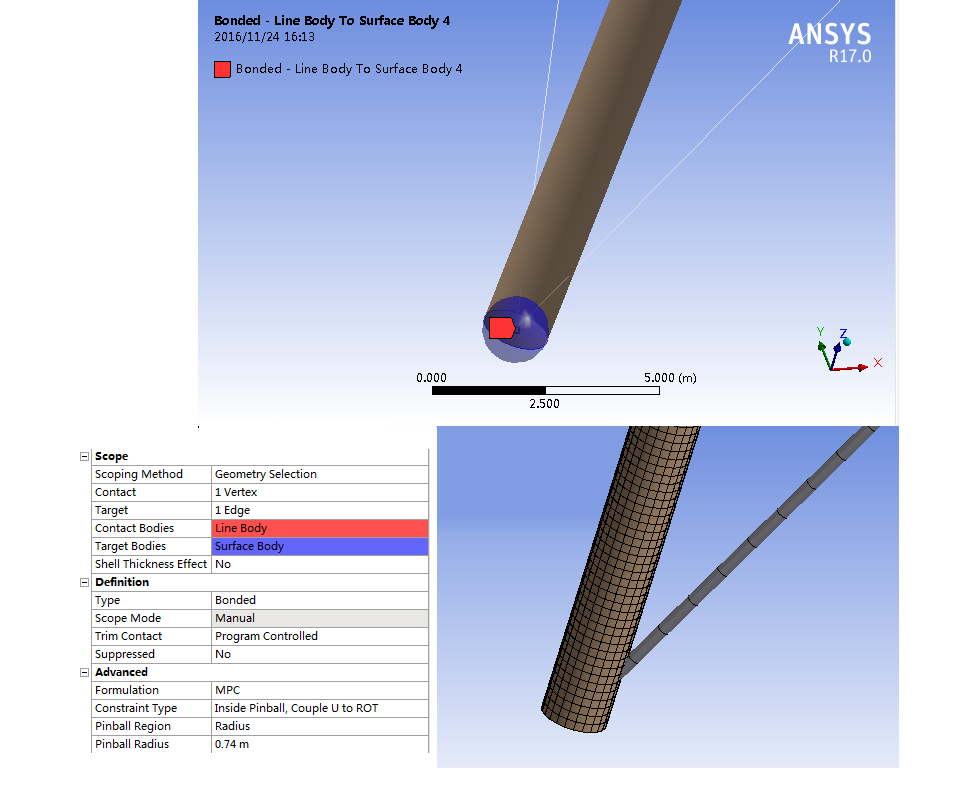
\includegraphics[width=0.8\textwidth]{mpc.png}
  \caption{结构多尺度模型}
  \label{fig:mpc}
\end{figure}

\subsection{数值模拟结果}

\begin{figure}[!htpb]
  \centering
  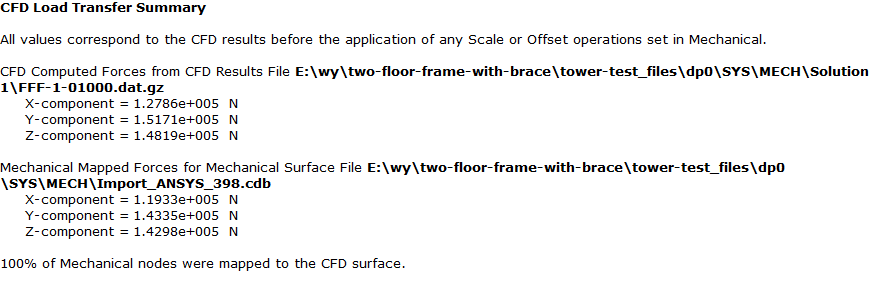
\includegraphics[width=0.8\textwidth]{load.png}
  \caption{流场压力导入说明}
  \label{fig:load}
\end{figure}

\begin{figure}[!htpb]
  \centering
  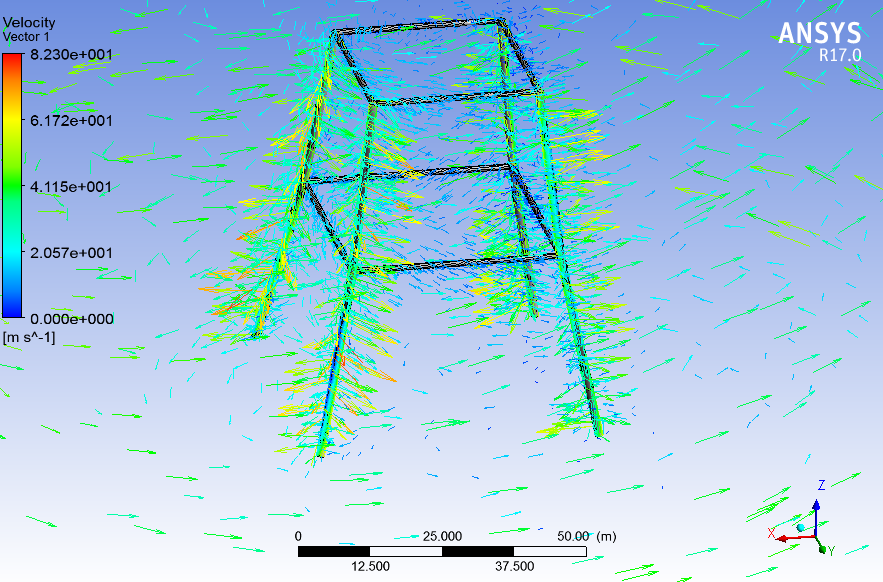
\includegraphics[width=0.8\textwidth]{velocity.png}
  \caption{结构周围流场速度矢量图}
  \label{fig:velocity}
\end{figure}

\begin{figure}[!htpb]
  \centering
  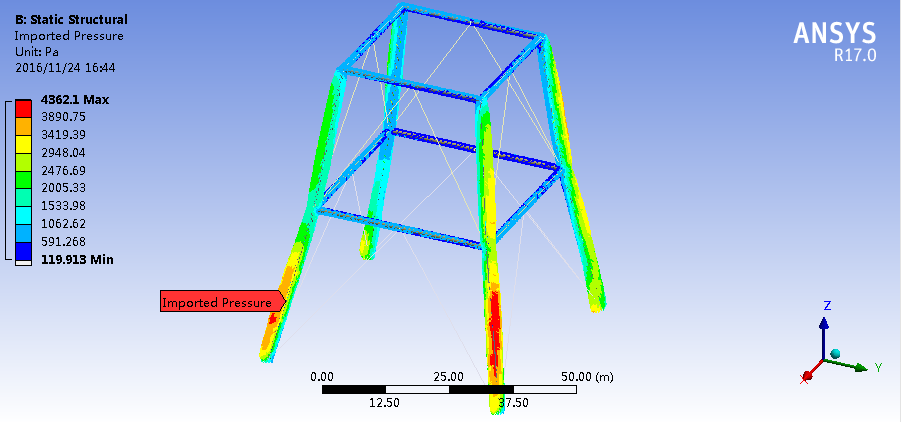
\includegraphics[width=0.8\textwidth]{pressure.png}
  \caption{结构表面所受风压}
  \label{fig:pressure}
\end{figure}

\begin{figure}[!htpb]
  \centering
  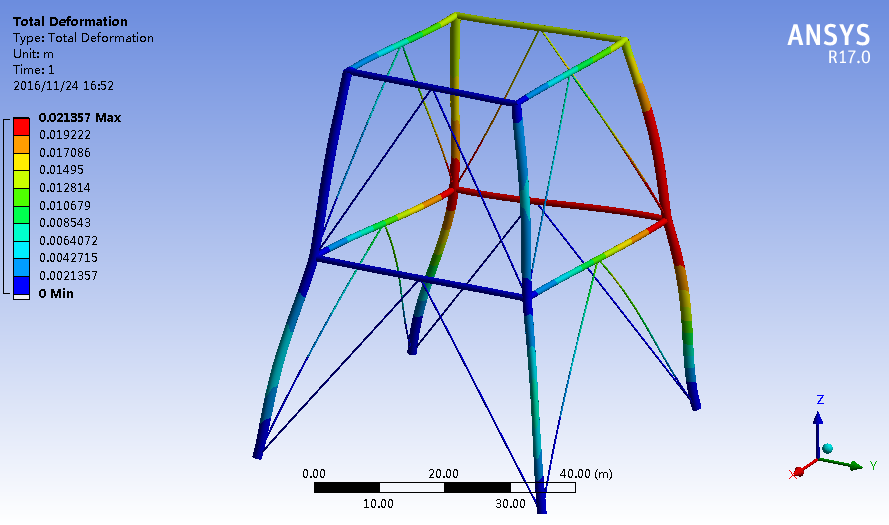
\includegraphics[width=0.8\textwidth]{disp.png}
  \caption{结构在龙卷风作用下变形云图}
  \label{fig:disp}
\end{figure}

\newpage
\bibliographystyle{seuthesix}
\bibliography{main}

\end{document}